\documentclass[a4paper, 12pt, twoside]{report}

% This can be used if you want to increase the spacing between lines to 1.5x
%\linespread{1.5}

%General packages

% Uncomment the following line for preparing the final hardcopy (and comment out the next one)
%\usepackage[a4paper,left=40mm,right=20mm,top=30mm,bottom=20mm]{geometry}
% Use this for your draft (easier to read). Don't forget to manually check
% everything when you switch to final hardcopy geometry (see above)
\usepackage[a4paper,left=20mm,right=20mm,top=30mm,bottom=20mm]{geometry}

\usepackage[utf8]{inputenc}
\usepackage{graphicx}
\usepackage{gensymb}
\usepackage{textcomp}
\usepackage{amsfonts}
\usepackage{appendix}
\usepackage{listings}
%\lstset{breaklines=true}
%\DeclareGraphicsExtensions{.pdf,.jpeg,.png}
\usepackage{amsmath}
\usepackage{amssymb}
\usepackage{algpseudocode}
\usepackage{algorithm}
%\usepackage{array}
\usepackage{subfig}
%\usepackage{captcont}
\usepackage{booktabs}
\usepackage[hyphens]{url}
\usepackage{multirow}
\usepackage{parskip}
%\usepackage{cite}
\usepackage[table]{xcolor}
\usepackage{hyperref}
\usepackage{amsfonts}
\usepackage{amsthm}
\usepackage{mathrsfs}
\usepackage{tikzit}

\input{figures/graphstyle.tikzstyles}

\newtheorem*{theorem*}{Theorem}
\newtheorem{theorem}{Theorem}[section]

\theoremstyle{definition}
\newtheorem{definition}{Definition}[section]
\newtheorem{exmp}{Example}[section]

\theoremstyle{remark}
\newtheorem*{rem}{Remark}

\def\NN{\ensuremath{\mathbb{N}}}
\def\N{\ensuremath{\mathbb{N}}}
\def\ZZ{\ensuremath{\mathbb{Z}}}
\def\Z{\ensuremath{\mathbb{Z}}}
\def\QQ{\ensuremath{\mathbb{Q}}}
\def\Q{\ensuremath{\mathbb{Q}}}
\def\RR{\ensuremath{\mathbb{R}}}
\def\R{\ensuremath{\mathbb{R}}}
\def\CC{\ensuremath{\mathbb{C}}}
\def\FF{\ensuremath{\mathbb{F}}}
\def\Pr{\ensuremath{\mbox{Pr}}}
%\newsavebox{\imagebox}

%Formatting for headers and footers
\usepackage{fancyhdr}
\pagestyle{fancy}
\fancyhead{}
%\fancyhead[RO,LE]{Monolithic Nanocomposite Detector for LaBrAT-PET}
\renewcommand{\headrulewidth}{0pt}
\fancyfoot{}
\fancyfoot[LE,RO]{\thepage}
%\fancyfoot[LO,RE]{Student Name}

%Bibliography settings
\usepackage[backend=biber,sorting=none,style=ieee]{biblatex}
\addbibresource{library.bib}

%Link to graphics folder
\graphicspath{{figures/}}

% Set your thesis title and author details here
\title{Random Numerical Semigroups}
\author{Santiago Morales Duarte}
\date{\today}

\begin{document}

\begin{titlepage}
\begin{center}
%\vspace*{1cm}

\Huge
\makeatletter
\textbf{\@title}

\Large

\vspace{3.cm}

by \textbf{\@author{}}

\vfill
\large
Thesis submitted in fulfilment of the requirements for the degree of\\
\textit{Bachelor of Science}\\
under the supervision of Tristram Bogart\\
\vfill
\large
Department of Mathematics\\
Faculty of Science\\
Universidad de los Andes\\

\today
\makeatother

\end{center}
\end{titlepage}


% \chapter*{Certificate of Authorship / Originality}

\makeatletter

I, \@author{}, declare that this thesis is submitted in fulfilment of the requirements for the award of Doctor of Philosophy, in the School of Electrical and Data Engineering at the University of Technology Sydney.
\makeatother

\vspace{6pt}

\noindent This thesis is wholly my own work unless otherwise referenced or acknowledged. In addition, I certify that all information sources and literature used are indicated in the thesis. This document has not been submitted for qualifications at any other academic institution.

% If applicable, the above statement must be replaced with the collaborative doctoral degree statement (see below).

% If applicable, the Indigenous Cultural and Intellectual Property (ICIP) statement must be added (see below).

\vspace{6pt}

\noindent This research is supported by the Australian Government Research Training Program.

% If you have a top-up or other scholarship, please modify this.

\vspace{1cm}

\begin{tabular}{m{3cm}m{7cm}}
Signature: &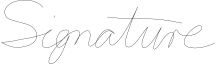
\includegraphics[width=6cm]{example_signature}\\

Date:	&\today\\
\end{tabular}
\vspace{6pt}

\makeatletter

% Can also use a copyright statement as below
%\hfill $\copyright$ Copyright \today{} \@author{}

\makeatother


\pagenumbering{roman}

\chapter*{Abstract}

This is the text of the abstract, providing a brief summary of the context, research problem, main contributions and conclusions of this work.


\chapter*{Dedication}

To my parents, for always loving and supporting me. 
To Mrtn Prd Grr


\chapter*{Acknowledgements}

I would like to thank (supervisor, family, research collaborators, anyone else who significantly helped you with this work).

{
\makeatletter
\vspace{1cm}
\raggedleft
\@author{}\\
\today{}\\
Bogotá, Colombia\\
\raggedright
\makeatother
}


\tableofcontents
\listoffigures
\listoftables

\pagenumbering{arabic}

% Add additional chapters as required
\chapter{Introduction}\label{chap:intro}

The start of the introduction provides some context and brief background.

\section{Research Objectives and Overview}

% There is some flexibility about how this is structured. This should be agreed with your supervisor as appropriate for your discipline!

The research question which this Thesis aims to answer is...

% Note that this could also be phased as a hypothesis to be validated.

The specific research objectives of this Thesis are:

\begin{enumerate}
\item Objective 1
\item Objective 2
\end{enumerate}

Chapter \ref{chap:litrev} provides a comprehensive review of literature which is relevant to the overall aim. This includes ...

Chapter \ref{chap:contrib1} aims to ...

This chapter resulted in the following publications:

\begin{itemize}
\item \fullcite{thesis_template}
\item \fullcite{thesis_template}
\end{itemize}

Chapter \ref{chap:contrib2} aims to ...

This chapter resulted in the following publications:

\begin{itemize}
\item \fullcite{thesis_template}
\end{itemize}

Chapter \ref{chap:contrib3} aims to ...

This chapter resulted in the following publications:

\begin{itemize}
\item \fullcite{thesis_template}
\end{itemize}

Finally, Chapter \ref{chap:conclusion} summarises the results and implications of this work, and provides recommended directions for continuation of this work in the future.

\subsection{Additional Research Contributions}

% Any additional research outputs - this could include invited talks, co-authored research outputs with minor contributions etc.

A number of additional research publications and presentations are listed below:

\begin{itemize}
\item xxx
\end{itemize}


Test \cite{thesis_template}

\chapter{The Probabilistic Method}\label{chap:probmet}

\section{Introduction}\label{sec:probmet:intro}

The probabilistic method is a powerful tool, with applications in Combinatorics, Graph Theory, Number Theory and Computer Science. It is a nonconstructive method that proves the existence of an object with a certain property, by showing that the probability that a randomly chosen object has that property is greater than zero. The method requires an appropiate sample space and is best illustrated by an example: \par

\begin{definition}\label{def:tournament}
A \textit{tournament} is a directed graph $T$ on $n$ vertices such that for every pair of vertices $i, j \in V(T)$, exactly one of the edges $(i, j)$ or $(j, i)$ is in $E(T)$. \cite{alon2016probabilistic} 
\end{definition}

The name of a tournament comes from the fact that it can be thought of as a sports tournament where each vertex represents a team and each team plays every other team exactly once. The edge $(i, j)$ represents a win for team $i$ over team $j$. A tournament $T$ has property $S_k$ if for every subset $K \subseteq V(T)$ of size $k$, there is a vertex $v \in V(T)$ such that $(v, s) \in E(T)$ for all $s \in K$ \cite{alon2016probabilistic}. That is, for every set of $k$ teams there is a team that beats all of them. For example, the tournament in Figure \ref{fig:tournament} has property $S_1$ since every team is beaten by another team. \par

A natural question to ask is: is there a tournament with property $S_k$ for every $k$? The answer is yes. We will prove this using the probabilistic method. First we define a probability space over the set of tournaments on $n$ vertices: \par 
A \textit{random} tournament on a set of $n$ vertices is a tournament $T$ such that for every pair of vertices $i, j \in V(T)$, the edge $(i, j)$ is in $E(T)$ with probability $\frac{1}{2}$ and the edge $(j, i)$ is in $E(T)$ with probability $\frac{1}{2}$, independently of all other edges. Thus, every tournament on $n$ vertices has the same probability, which means that this probability space is \textit{symmetric}. \par

\begin{figure}
    \centering
    \[\begin{tikzcd}
        & \bullet \\
        \\
        \bullet && \bullet
        \arrow[from=3-1, to=1-2]
        \arrow[from=1-2, to=3-3]
        \arrow[from=3-3, to=3-1]
    \end{tikzcd}\]
    \caption{A tournament on 3 vertices with property $S_1$.}
    \label{fig:tournament}
\end{figure}

The main idea is to show that there is a large $n$ as a function of $k$, such that the probability that a random tournament on $n$ vertices has property $S_k$ is greater than zero. This implies that there is at least one tournament with property $S_k$. \par


\begin{theorem}
    For every $k \in \N$, there is a tournament with property $S_k$. \cite{alon2016probabilistic}
\end{theorem}

\textbf{Proof. } Fix a subset $K \subseteq V(T)$ of size $k$. Consider the event $A_K$ that there is no vertex $v \in V(T)$ such that $(v, s) \in E(T)$ for all $s \in S$. For any vertex $v \in V(T) \setminus K$, the probability that $(v, s) \notin E(T)$ for all $s \in K$ is $2^{-k}$. Thus,
\[\Pr[A_K] = \left(1 - 2^{-k}\right)^{n - k}.\]
Now, if we consider all subsets $S \subseteq V(T)$ of size $k$, then the probability that $T$ does not have property $S_k$ is the probability that any of the events $A_S$ occurs. Since there are $\binom{n}{k}$ such subsets, by the union bound,
\[\Pr\left[\bigvee_{\substack{S \subseteq V(T) \\ |S| = k}} A_S\right] \leq \sum_{\substack{S \subseteq V(T) \\ |S| = k}}\Pr[A_K] = \binom{n}{k}\left(1 - 2^{-k}\right)^{n - k}.\]
We want to show that, for some $n$, this probability of this event is less than 1. Using Propositions \ref{ap:prop:upperbinom} and \ref{ap:prop:exp}, we have that
\begin{align}
    \Pr\left[\bigvee_{\substack{S \subseteq V(T) \\ |S| = k}} A_S\right] &\leq \binom{n}{k}\left(1 - 2^{-k}\right)^{n - k} \\
    &\leq \left(\frac{en}{k}\right)^k\left(e^{-2^{-k}}\right)^{n - k} = e^{k\log\left(\frac{n}{k}\right) - \frac{n - k}{2^k}}. \label{eq:tournament}
\end{align}
Then, \ref{eq:tournament} is less than one if 
\[k\log\left(\frac{n}{k}\right) - \frac{n - k}{2^k} = k\log n - k\log k + \frac{k}{2^k} - \frac{n}{2^k} < k\log n - \frac{n}{2^k} < 0,\]
which holds if and only if
\[\frac{n}{\log n} > k2^k.\]
Now, if $n = k^2 2^k\log 2$, then
\[\lim_{n \to \infty} \frac{n}{k2^k\log n} = \lim_{k \to \infty} \frac{k\log 2}{2\log k + k\log 2 + \log\log 2} = 1.\]
Hence, we conclude that there exists $n = (\log 2)k^2 2^k (1 + o(1))$, such that the probability that a random tournament on $n$ vertices does not have property $S_k$ is less than one. Therefore, the probability that there exists a tournament on $n$ vertices with property $S_k$ is greater than zero, which means that there exists at least one tournament with property $S_k$. \qed

We make two observations: 
\begin{enumerate}
    \item We used the \textit{union bound}. The union bound is a common technique in the probabilistic method. It states that for any events $A_1, ..., A_n$,
    \[\Pr[A_1 \cup ... \cup A_n] \leq \Pr[A_1] + ... + \Pr[A_n].\]
    We will extensively use this technique in this thesis. In a measure space, the union bound is the same property as \textit{subadditivity}. \par
    \item The proof is nonconstructive. It does not give us a way to find a tournament with property $S_k$. It only shows that there is at least one. This is a common feature of the probabilistic method. However, in this case, we have that for large enough $n$, the probability that a random tournament on $n$ vertices has property $S_k$ is close to one. This means that we can find a tournament with property $S_k$ by generating random tournaments until we find one with the desired property. If $n$ is large enough, this will not take too long. \par
\end{enumerate}
In this chapter, we will introduce some tools that are useful for applying the probabilistic method. We will also give some examples of the method in action. \par

\section{Linearity of Expectation}\label{sec:probmet:linearity}

Let $X_1, \ldots, X_n$ be random variables. Linearity of expectation states that 
\[E[c_1X_1 + \cdots + c_nX_n] = c_1E[X_1] + \cdots + c_2E[X_2].\]
Note that the variables do not need to be independent. Also, in a probability space, there is a point for which $X \geq E[X]$ and there is \ref{def:tournament}

\section{Second Moment Method}\label{sec:probmet:secondmoment}

\section{Threshold Functions}\label{sec:probmet:threshold}

Let $n \in \N$ and $0 \leq p \leq 1$. The random graph $G(n, p)$ is a probability space over the set of graphs on $n$ labeled vertices determined by
\[\Pr[\{i, j\} \in G] = p\] 
with these events mutually independent \cite{alon2016probabilistic}. Given a graph theoretic property $A$, there is a probability that $G(n, p)$ satisfies $A$, which we write as $\Pr[G(n, p) \vDash A]$. 

\begin{definition}
    $r(n)$ is a threshold function for a graph theoretic property $A$ if 
    \begin{enumerate}
        \item When \(p(n) \in o(r(n)), \; \lim_{n \to \infty} \Pr[G(n, p(n)) \vDash A] = 0,\)
        \item When \(r(n) \in o(p(n)), \;  \lim_{n \to \infty} \Pr[G(n, p(n)) \vDash A] = 1,\) 
    \end{enumerate}
    or vice versa. \cite{alon2016probabilistic}
\end{definition}

We give an example of a threshold function which illustrates a common method for proving that a function is a threshold. \par

\subsection{Threshold function for having isolated vertices}

Let $G$ be a graph on $n$ labeled vertices. An isolated vertex of $G$ is a vertex which does not belong to any of the edges of $G$. Let $A$ be the property that $G$ contains an isolated vertex. We will prove that $\displaystyle{r(n) = \frac{\ln n}{n}}$ is a threshold for $A$. \par

For each vertex $i$ in $G$ define the variable 

\[X_i = 
\left\{
	\begin{array}{ll}
		1  & \mbox{if } i \text{ is an isolated vertex,} \\
		0 & \mbox{if } i \text{ is not an isolated vertex.}
	\end{array}
\right.
\]

Now, the probability that a vertex $i$ is isolated is $(1 - p)^{n - 1}$ since it is the probability that none of the other $n - 1$ vertices is connected to $i$. Let $X = \sum_{i = 1}^n X_i$, then the expected number of isolated vertices is
 \[E[X] = \sum_{i = 1}^{n} E[X_i] = \sum_{i = 1}^{n} \Pr[X_i] = n(1 - p)^{n - 1}.\]

Let $\displaystyle{p = k\frac{\ln n}{n}}$ for $k \in \R_{>0}$. Then
\begin{align*}
    \lim_{n \to \infty} E[X] &= \lim_{n \to \infty} n\left(1 - k\frac{\ln n}{n}\right)^{n - 1} \\
    &= ne^{-k\ln n} = n^{1 - k}.
\end{align*}

Therefore, $\lim_{n \to \infty} E[X] = 0$ if $k > 1$. Since \(E[X] \geq \Pr[X > 0],\) we conclude that \[\lim_{n \to \infty} \Pr[G(n, p) \vDash A] =  \lim_{n \to \infty} \Pr[X > 0] = 0.\] \par
Now, for $k < 1$, the fact that $\lim_{n \to \infty} E[X] = \infty$ is not enough to conclude that \(\lim_{n \to \infty} \Pr[G(n, p) \vDash A] = 1\). We have to use the second moment method. \par

\begin{theorem*}
    If $E[X] \to \infty$ and $\text{Var}[X] = o(E[X]^2)$, then $\lim_{n \to \infty} \Pr[X > 0] = 1$. \cite{alon2016probabilistic}
\end{theorem*}

\textbf{Proof. } We will prove that, in this case, $Var[X] = o(E[X]^2)$. First, 
\begin{align*}
    \sum_{i \neq j}E[X_iX_j] &= \sum_{i \neq j} \Pr[X_i = X_j = 1] \\
    &= n(n - 1)(1 - p)^{n -1}(1 - p)^{n - 2} \\ &= n(n - 1)(1 - p)^{2n - 3},
\end{align*}

for if $i$ is an isolated vertex, then there is no edge between $i$ and $j$ so we only have to account for the remaining $n - 2$ edges that contain $j$.  \par

Thus, since $\sum_{i = 1}^{n}E[X_i^2] =  \sum_{i = 1}^n E[X_i] = E[X]$ and $\lim_{n \to \infty} p = 0$,

\begin{align*}
    \lim_{n \to \infty} \frac{\text{Var}[X]}{E[X]^2} &= 
    \lim_{n \to \infty}\frac{E[X^2] - E[X]^2}{E[X]^2} = \lim_{n \to \infty} \frac{\sum_{i = 1}^n E[X_i^2] + \sum_{i \neq j}E[X_iX_j]}{E[X]^2} - 1 \\ &= 0 + \lim_{n \to \infty} \frac{ n(n - 1)(1 - p)^{2n - 3}}{n^2(1 - p)^{2n - 2}} - 1= \lim_{n \to \infty} \frac{1}{1 - p} - 1 = 0.\\
\end{align*} \par
We conclude that $\text{Var}[X] \in o(E[X]^2)$ and so, if $k < 1$, \[\lim_{n \to \infty} \Pr[G(n, p) \vDash A] = \lim_{n \to \infty} \Pr[X > 0] = 1.\] Therefore, $r(n) = \frac{\ln n}{n}$ is a threshold function for property $A$.


\chapter{Numerical Semigroups}\label{chap:smgs}

\section{Introduction}\label{sec:smgps:intro}

So far we have only discussed graphs. In this chapter, we will introduce a new object which has a different structure, but for which the probabilistic method can be used to prove results. \par

\begin{definition} \cite{rosales2009numerical}
    A \textit{numerical semigroup} is a subset $S \subseteq \NN_{0}$ for which 
    \begin{enumerate}
        \item $0 \in S$,
        \item $S$ is closed under addition, i.e. $a, b \in S$ implies $a + b \in S$, and
        \item $S$ has finite complement in $\NN_{0}$.
    \end{enumerate}
\end{definition}

Examples of numerical semigroups include $\NN_{0}$ and $\NN_{0} \setminus \{1\}$. Subsets of $\NN_0$ which are not numerical semigroups include the set of even numbers, any finite set and $\NN_0 \setminus \{2\}$. \par

\begin{example}\label{ex:smgps:mcnugget}
    The \textit{McNugget Semigroup} is the set of all non-negative integers which can be expressed as a sum of non-negative multiples of 6, 9 and 20. 
\end{example}

Suppose you are in the United Kingdom and you wish to order 43 McNuggets. The cashier will hesitate for a while before telling you that they do not sell 43 McNuggets. However, if you order 44 McNuggets, you will receive 2 boxes of 20 McNuggets and 2 boxes of 2 McNuggets. This is because 44 can be expressed as a sum of non-negative multiples of 6, 9 and 20, namely $44 = 2 \cdot 6 + 2 \cdot 9 + 2 \cdot 20$ \cite{youtube}. 

Let us see why the McNugget Semigroup is a numerical semigroup. First, we note that $0$ can be expressed as a sum of non-negative multiples of 6, 9 and 20, namely $0 = 0 \cdot 6 + 0 \cdot 9 + 0 \cdot 20$. Next, we note that if $a$ and $b$ can be expressed as a sum of non-negative multiples of 6, 9 and 20, then so can $a + b$. Finally, we note that the complement of the McNugget Semigroup in $\NN_0$ is finite, since any integer greater than or equal to 43 can be expressed as a sum of non-negative multiples of 6, 9 and 20. \par

\section{Invariants}\label{sec:smgps:theme1}

\begin{definition}[Multiplicity]
    
\end{definition}



\begin{definition}[Embedding Dimension]
\end{definition}

\begin{definition}[Apéry Set]
\end{definition}

\begin{definition}[Frobenius Number]

\end{definition}


\begin{definition}[Genus]

\end{definition}

\section{Wilf's Conjecture}\label{sec:smgps:theme2}

Etc. etc.


% All contribution chapters should follow a similar structure, with a
% mini-introduction and overview at the beginning and a conclusion at the
% end bookmarking a structured presentation of the contribution. This can be
% largely based on your publications.

\chapter{Random Numerical Semigroups}\label{chap:randnumsems}

\section{Box Model}\label{sec:randomsmpgs:intro}

\begin{algorithm}
\caption{An algorithm with caption}\label{alg:cap}
\begin{algorithmic}
\Require $n \geq 0$
\Ensure $y = x^n$
\State $y \gets 1$
\State $X \gets x$
\State $N \gets n$
\While{$N \neq 0$}
\If{$N$ is even}
    \State $X \gets X \times X$
    \State $N \gets \frac{N}{2}$  \Comment{This is a comment}
\ElsIf{$N$ is odd}
    \State $y \gets y \times X$
    \State $N \gets N - 1$
\EndIf
\EndWhile
\end{algorithmic}
\end{algorithm}

\subsection{Results}\label{sec:contrib1:theme1:B}

\subsection{Subtopic C}\label{sec:contrib1:theme1:C}

\section{ER-type model}

We generate a random numerical semigroup with a model similar to the Erdös-Rényi model for random graphs. 

\begin{definition}
    For $p \in [0, 1]$ and $M \in \NN$, a random numerical semigroup $S(M, p)$ is a probability space over the set of semigroups $S = \langle\mathcal{A}\rangle$ with $\mathcal{A} \subseteq \{1,...,M\}$, determined by
    \[\Pr[n \in \mathcal{A}] = p,\]
    with these events mutually independent.
\end{definition}

\section{Downward model}\label{sec:contrib1:theme2}

Etc. etc.



\section{Conclusion}


% All contribution chapters should follow a similar structure, with a
% mini-introduction and overview at the beginning and a conclusion at the
% end bookmarking a structured presentation of the contribution. This can be
% largely based on your publications.

\chapter{Experiments}\label{chap:experiments}

\section{ER-type model experiments}

We used the following algorithm for random numerical semigroup generation. 

\begin{algorithm}
    \caption{An algorithm with caption}\label{alg:cap}
    \begin{algorithmic}
    \Require $n \geq 0$
    \Ensure $y = x^n$
    \State $y \gets 1$
    \State $X \gets x$
    \State $N \gets n$
    \While{$N \neq 0$}
    \If{$N$ is even}
        \State $X \gets X \times X$
        \State $N \gets \frac{N}{2}$  \Comment{This is a comment}
    \ElsIf{$N$ is odd}
        \State $y \gets y \times X$
        \State $N \gets N - 1$
    \EndIf
    \EndWhile
    \end{algorithmic}
\end{algorithm}
    
For random sums of cyclic groups, we used the following algorithm.

In this Chapter, XXX is presented. Include pseudocode. 
..

\section{Downward model experiments}\label{sec:experiments:downward model}

Etc. etc.



\chapter{Results}\label{chap:results}


\section{Introduction}  

In this chapter, we present the main results of this thesis. We will prove a theorem similar to parts (b) and (c) of Theorem \ref{thm:ermodel} using standard probabilistic arguments. 

\begin{theorem}\label{thm:main}
    Let $\mathcal{S} \sim \mathcal{S}(M, p)$, where $p = p(M)$ is a monotone decreasing function of $M$ and $\frac{1}{M} \in o(p(M))$. Then, 
\begin{enumerate}[label=(\alph*)]
    \item If $\lim_{M \to \infty} p(M) = 0$, then for every $K \in \N$,   
    \[\lim_{M \to \infty} \Pr[e(\mathcal{S}) > K] = \lim_{M \to \infty} \Pr[g(\mathcal{S}) > K] = \lim_{M \to \infty} \Pr[F(\mathcal{S}) > K] = 1.\]
    \item If $\lim_{M \to \infty} p(M) > 0$, then $e(\mathcal{S}), \; g(\mathcal{S})$ and $F(\mathcal{S})$ are bounded in probability, i.e., for every $\varepsilon > 0$, there exists $K_\varepsilon$ such that 
    \[ \Pr[e(\mathcal{S}) < K_\varepsilon] > 1 - \varepsilon, \quad  \Pr[g(\mathcal{S}) < K_\varepsilon] > 1- \varepsilon \quad \text{and} \quad \Pr[F(\mathcal{S}) < K_\varepsilon] > 1 - \varepsilon.\]
\end{enumerate}
Furthermore, there exists $K \in \NN$ such that
\begin{align*}
\lim_{p \to 0}\Pr\left[F(\mathcal{S}) \leq \frac{K}{p}\left(\log \frac{1}{p}\right)^3\right] &= \lim_{p \to 0}\Pr\left[g(\mathcal{S}) \leq \frac{K}{p}\left(\log \frac{1}{p}\right)^3\right]  
\\&= \lim_{p \to 0}\Pr\left[e(\mathcal{S}) \leq 3K\left(\log \frac{1}{p}\right)^3\right] = 1.
\end{align*}
\end{theorem}
We will also show that that this Theorem is \textit{stronger} than Theorem \ref{thm:ermodel}. The proof of part (b) of this theorem is based on Lemma \ref{lem:sumset}, which is a result on sums of random subsets of cyclic groups.  

\section{Lower Bound}\label{sec:results:lowerbound}

We first prove part (a) of Theorem \ref{thm:main}. We will show that, for each fixed number of generators $a$, there is a high probability that at least $a$ minimal generators are chosen as $p \to 0$.

\textbf{Proof. }
Fix $a \in \NN$ such that $a > 11$ and let $T = \{1, \ldots, \lfloor\frac{a}{p}\rfloor\}$. Since   $\frac{1}{M} \in o(p)$, we have that $\lfloor\frac{a}{p}\rfloor \leq M$ for large enough $M$. Consider the following events:
\begin{itemize}
    \item $E_1$: No generator selected is less than $\frac{1}{ap}$.  \par
    Let $X_1$ be the number of generators selected from $\{1,\ldots,\lfloor\frac{1}{ap}\rfloor\}$. Then 
    \begin{equation}\label{eq:lowerbound:e1}
    \Pr[\lnot E_1] = \Pr[X_1 > 0] \leq \EE[X_1] \leq p \cdot \frac{1}{ap} = \frac{1}{a}.
    \end{equation}

    \item $E_2:$ At most $\frac{3a}{2}$ generators are selected from $T$.\par 
    Let $X_2$ be the number of generators selected in $T$, then $X_2 \sim \mathrm{Bin}(\frac{a}{p}, p)$ and we can use the bound in Proposition \ref{ap:prop:rightbinomtail} with $r = \frac{3a}{2}$ to get that

    \[\Pr[\lnot E_2] = \Pr\left[X_2 > \frac{3a}{2}\right] \leq  \frac{\frac{3a}{2}(1 - p)}{(\frac{3a}{2} - a)^2} = \frac{\frac{3a}{2}(1 - p)}{(\frac{a}{2})^2}\leq \frac{6}{a}.\]

    Also, by the union bound and (\ref{eq:lowerbound:e1}),
    \begin{equation}\label{eq:lowerbound:e1ande2}
     \Pr[E_1\land E_2] \geq 1 - \frac{1}{a} - \frac{6}{a} = 1 - \frac{7}{a}.
    \end{equation}

    \item $E_3:$ At least $\frac{a}{2}$ generators are selected from $T$. \par 
    Similarly, we can use the bound for the left tail (Proposition \ref{ap:prop:leftbinomtail}) with $r = \frac{a}{2}$ to get that
    \begin{equation}\label{eq:lowerbound:e3}
        \Pr[ \lnot E_3] = \Pr\left[X_2 < \frac{a}{2}\right] \leq  \frac{(n - \frac{a}{2})p}{(np - \frac{a}{2})^2} = \frac{a - (\frac{a}{2})p}{(\frac{a}{2})^2} \leq \frac{4}{a}.
    \end{equation}
    \item $E_4:$ The generators selected from $T$ are all minimal.\par 
    Let $A_T = \{Y_{(1)}, Y_{(2)}, \ldots, Y_{(k)}\}$ be the generators selected in $T$ in order. Assume $E_1$ and $E_2$. We have that $E_1$ implies $Y_{(1)} \geq \frac{1}{ap}$ and $E_2$ implies $k \leq \frac{3a}{2}$. \par
    First we bound the probability that $b \in T$ is selected as a generator. Using conditional probability, we have that 
    \begin{align}
        \Pr[b \in \mathcal{A}_T|E_1 \land E_2] &= \frac{\Pr[(b \in \mathcal{A}_T)\land E_1 \land E_2]}{\Pr[E_1 \land E_2]} \\
        &\leq\frac{\Pr[b \in \mathcal{A}_T]}{\Pr[E_1 \land E_2]} = \frac{p}{1 - \frac{7}{a}}. \label{eq:lowerbound:inequality}
    \end{align}
    Now, if no multiple of $Y_{(1)}$ is selected in $T$, then $Y_{(2)}$ is minimal. Thus, $Y_{(2)}$ is minimal if $\langle y_1 \rangle \cap  \mathcal{A}_T = \{y_1\}$. Also, note that, since the generators are chosen independently,
    \[P[b \in \mathcal{A}_T] = P[b \in \mathcal{A}_T|Y_{(1)} = y_1] \quad \text{if} \quad  b > y_1.\]
    Since $y_1 \geq \frac{1}{ap}$, we have that \[|\langle y_1 \rangle \cap  \mathcal{A}_T| \leq |\langle y_1 \rangle \cap T| \leq a^2.\] Then, using the union bound and (\ref{eq:lowerbound:inequality}),
    \begin{align*}
        \Pr[Y_{(2)} \text{ is not minimal}|E_1\land E_2 \land Y_{(1)} = y_1]&\leq \sum_{b \in\langle y_1\rangle \cap T}\Pr[b \in \mathcal{A}_T|E_1 \land E_2 \land Y_{(1)} = y_1]\\ 
        &\leq \sum_{b \in\langle y_1\rangle \cap T} \frac{p}{1 - \frac{7}{a}} \leq \frac{pa^2}{1 - \frac{7}{a}}.
    \end{align*}
        
    If this bound is independent of $y_1$, we get that 
    \begin{equation}\label{eq:lowerbound:y2notminimal}
        \Pr[Y_{(2)} \text{ is not minimal}|E_1\land E_2] \leq \frac{pa^2}{1 - \frac{7}{a}}.
    \end{equation}
    Similarly, for $2 \leq t \leq k$ and fixed $Y_{(1)} = y_1, \ldots, Y_{(t - 1)} = y_{t - 1}$, $Y_{(t)}$ is minimal if $\langle y_1, \ldots, y_{t - 1}\rangle \cap \mathcal{A}_T = \{y_1, \ldots, y_{t - 1}\}$. To bound $|\langle y_1, \ldots, y_{t - 1}\rangle \cap \mathcal{A}_T|$, there are at most $a^2$ choices for each multiple of $y_i$, so there are at most $a^{2(t - 1)}$ such linear combinations and
    \[|\langle y_1, \ldots, y_{t - 1} \rangle \cap  \mathcal{A}_T| \leq |\langle y_1, \ldots, y_{t - 1} \rangle \cap T| \leq a^{2(t - 1)}.\]
    Also, 
    \[P[b \in \mathcal{A}_T] = P[b \in \mathcal{A}_T|Y_{(1)} = y_1\land \cdots \land Y_{(t - 1)} = y_{t - 1}] \quad \text{if} \quad  b > y_{t - 1} > \ldots > y_1,\]
    and so
    \[
        \Pr[b \in \mathcal{A}_T|E_1 \land E_2 \land Y_{(1)} = y_1 \land \cdots \land Y_{(t - 1)} = y_{t - 1}] \leq \frac{p}{1 - \frac{7}{a}}.
    \]
    Then, as in (\ref{eq:lowerbound:y2notminimal}), 
    \[\Pr[Y_{(t)} \text{ is not minimal}|E_1\land E_2] \leq \frac{pa^{2t}}{1 - \frac{7}{a}} .\]
    Therefore, we can use the union bound and $k \leq \frac{3a}{2}$ to conclude that
    \[\Pr[E_4|E_1 \land E_2] \geq 1 - \frac{p}{1 - \frac{7}{a}}\sum_{t = 1}^{\frac{3a}{2} - 1}a^{2(t - 1)} = 1 - o(1),\]
    since $a$ is constant and $p \to 0$ as $M  \to \infty$.
    Thus,  
    \begin{equation}\label{eq:lowerbound:e4}
        \Pr[E_4] = \Pr[E_4| E_1 \land E_2]\Pr[E_1\land E_2] \geq 1 - \frac{7}{a} - o(1).
    \end{equation}
\end{itemize}


Finally, note that by the union bound, (\ref{eq:lowerbound:e3}) and (\ref{eq:lowerbound:e4}),
\[\Pr[E_4 \land E_3] \geq 1 - \frac{11}{a} - o(1).\] 
This means that for $\varepsilon > 0$ and sufficiently large $a$ and $M$, the probability that at least $\frac{a}{2}$ minimal generators are selected is greater than $1 - \varepsilon$. Threfore, for every $K \in \NN$, 
\[\lim_{M \to \infty} \Pr[e(\mathcal{S}) > K] = 1.\]
Now, using Corollary \ref{cor:smgps:embedding_dim} and Proposition \ref{prop:smgps:frobgenus}, we have that
\[e(S) \leq m(S) \leq g(S) + 1 \leq F(S) + 1.\]
We conclude that, for every $K \in \NN$,
\[\lim_{M \to \infty} \Pr[g(\mathcal{S}) > K] = \lim_{M \to \infty} \Pr[F(\mathcal{S}) > K] = 1.\qed\]

\section{Upper bound}\label{sec:results:upperbound}
Before proving part (b) of the Theorem \ref{thm:main}, we will prove a lemma that shows that a cyclic group of prime order is covered by the sums of a random subset of logarithmic size almost always.
\begin{lemma}\label{lem:sumset}
    Let $q$ be a prime number and $\mathcal{A}$ be a random subset of $\mathbb{Z}_q$ of size $4\lfloor6\log_2 q\rfloor$. As $q$ tends to infinity, $2\lfloor6\log_2 q\rfloor \mathcal{A}$ covers $\mathbb{Z}_q$ almost always. 
\end{lemma}

\textbf{Proof. } Let $s \in \mathbb{N}$ such that $s\leq q$. Let $\mathcal{A}$ be a uniformly random subset of $\mathbb{Z}_q$ of size $s$, that is, 
\[\Pr(\mathcal{A}) = \frac{1}{\binom{q}{s}}.\]
For a given $z \in \mathbb{Z}_q$ and $k \in \mathbb{N}$ for which $k \leq s/2$, let 
\[N_z^k := \left\{K \subseteq \mathbb{Z}_q: |K| = k, \sum_{t \in K} t = z\right\}.\]
Note that $|N_z^k| = \frac{1}{q}{\binom{q}{k}}$, since $K \in N_0^k$ if and only if $K + k^{-1}z \in N_z^k$ for every $z \in \mathbb{Z}_q$.\par
For $K \in N_z^k$, let $E_K$ be the event that $K \subset\mathcal{A}$. Let $X_K$ be the indicator variable of $E_K$.
We define the random variable 
\[X_z = \sum_{K \in N_z^k} X_K.\]
Note that $X_z$ counts the number of sets of size $k$ which add up to $z$. We now find $\EE[X_z]$. Since the sum of every subset $K \subset S$ is in $\mathbb{Z}_q$,
\[\sum_{z \in Z_q} X_z = {\binom{s}{k}},\]
and so
\[\binom{s}{k} = \EE\left[\sum_{z \in Z_q} X_z\right] =  \sum_{z \in Z_q} \EE[X_z].\]\par
As in the argument for finding $|N_z^k|$, for every $z \in \mathbb{Z}_q$, 
\[\EE[X_0] = \sum_{K \in N_0^k}\EE[X_K] = \sum_{K \in N_0^k} \EE[X_{K + k^{-1}z}] = \sum_{K \in N_z^k} \EE[X_K] = \EE[X_z].\]
Therefore, we have that
\begin{equation}\label{eq:upperbound:expected}
E[X_z] = \frac{1}{q} {\binom{s}{k}}.
\end{equation}
Now, for $K, L \in N_z^k$, let $j \in \mathbb{N}$ such that $j \leq k$ and define
\[\Delta_j := \sum_{|K \cap L| = j} \Pr[E_K \land E_L].\]
\par 
If $|K \cap L| = j$,
\[\Pr[E_K \land E_L] = \frac{\binom{q - 2k + j}{s - 2k + j}}{\binom{q}{s}}.\]
\par
We can bound the number of events for which $|K \cap L| = j$. First we choose $K$ as any set in $N_z^k$ and then we choose the remaining $k- j$ elements as any subset of $\mathbb{Z}_q \setminus K$ with size $k - j$. Thus, 
\[\Delta_j \leq \frac{1}{q}\binom{q}{k}\binom{q - k}{k - j} \frac{\binom{q - 2k + j}{s - 2k + j}}{\binom{q}{s}}.\]
\par This implies that, using \ref{eq:upperbound:expected},
\begin{align*}
    \frac{\Delta_j}{\EE[X_z]^2} &\leq \frac{\binom{q}{k} \binom{q - k}{k - j}\binom{q - 2k + j}{s - 2k + j}}{\frac{1}{q} \binom{s}{k}\frac{1}{q} \binom{s}{k}q\binom{q}{s}} \\
    &= \frac{\frac{q!}{(q - k)!k!}\frac{(q - k)!}{(k - j)!(q - 2k + k)!}\frac{(q - 2k + j)!}{(s - 2k + j)!(q - s)!}}{\frac{1}{q}\binom{s}{k}\frac{s!}{(s - k)!k!}\frac{q!}{(q - s)!s!}} \\
    &= \frac{q\binom{s - k}{k - j}}{\binom{s}{k}}.
\end{align*}
Let $s = 4\lfloor 6 \log_2 q \rfloor$ and $k = 2\lfloor 6 \log_2 q \rfloor$. Using that $\binom{s - k}{k - j}$ is maximized at $k - j = \lfloor (s - k) / 2\rfloor$,
\begin{align*}
\frac{\Delta_j}{\EE[X_z]^2} \leq \frac{q \binom{2\lfloor 6 \log_2 q \rfloor}{\lfloor 6 \log_2 q \rfloor}}{\binom{4\lfloor 6 \log_2 q \rfloor}{2\lfloor 6 \log_2 q \rfloor}} \leq \frac{q}{\binom{2\lfloor 6 \log_2 q \rfloor }{ \lfloor 6 \log_2 q \rfloor}} \leq \frac{q}{2^{\lfloor 6 \log_2 q \rfloor}} \sim \frac{1}{q^5},
\end{align*}
since \(\binom{2\lfloor 6 \log_2 q \rfloor}{\lfloor 6 \log_2 q \rfloor}^2 \leq \binom{4\lfloor 6 \log_2 q \rfloor }{2\lfloor 6 \log_2 q \rfloor}\) (Proposition \ref{ap:prop:binom}).   \par
Hence, by (\ref{eq:probmet:deltainequality}) and Theorem \ref{thm:probmet:secondmoment:1},
\begin{align*}
\Pr[X_z = 0] \leq \frac{\EE[X_z] + \Delta}{\EE[X_z]^2} &= \frac{1}{E[X_z]} + \sum_{j = 0}^k \frac{\Delta_j}{\EE[X_z]^2} \\
&\leq \frac{1}{E[X_z]} + \frac{(k + 1)}{q^5} = \frac{1}{E[X_z]} + \frac{2\lfloor 6 \log_2 q\rfloor + 1}{q^5}.
\end{align*}
Therefore, by the union bound and since $q \to \infty$ as $p \to 0$,
\begin{align}
\Pr\left[\bigvee_{z \in \mathbb{Z}_q} X_z = 0\right] &\leq \frac{q}{\EE[X_z]} + \frac{2\lfloor 6 \log_2 q \rfloor + 1}{q^4}\\
 &= \frac{q^2}{\binom{4\lfloor 6 \log_2 q \rfloor}{2\lfloor 6 \log_2 q \rfloor}} + \frac{2\lfloor 6 \log_2 q \rfloor + 1}{q^4} \\
 &\leq \frac{q^2}{2^{2\lfloor 6 \log_2 q \rfloor}} + \frac{2\lfloor 6 \log_2 q \rfloor + 1}{q^4} \\
 &\sim \frac{1}{q^{10}} + \frac{6\log q}{q^4}= o(1).\label{eq:lemma:prob}
\end{align}
We conclude that, as $q \to \infty$, $X_z > 0$ for every $z \in \mathbb{Z}_q$ almost always. Thus, for every $z \in \mathbb{Z}_q$, there exists $K \in N_z^k$ such that $K \subset \mathcal{A}$ almost always. This means that $2\lfloor 6 \log_2 q \rfloor \mathcal{A}$ covers $\mathbb{Z}_q$ almost always. \qed

\subsection{Proof of the upper bound} 
\begin{lemma}\label{lem:upperbound}
    Let $\psi(x)$ be a function for which $x(\log x)^2 \in o(\psi(x))$ .Then
    \[\lim_{p \to 0}\Pr\left[F(\mathcal{S}) \leq \psi\left(\frac{1}{p}\right)\right] = 1.\] 
\end{lemma}

\par The proof of this theorem consists of several parts. The strategy is to prove that the Ápery set of a subsemigroup of $S$ is completed before step $\psi\left(\frac{1}{p}\right)$ with high probability, since $F(\mathcal{S})$ is less than the maximum element of this Ápery set. The proof has the following structure: 
\begin{enumerate}
\item First, we will find a step for which a prime $q$ is chosen with high probability ($E_1$). 
\item Then, in the spirit of Lemma \ref{lem:sumset} we will find a step such that a set $\mathcal{A}$ of $s$ elements which are different modulo $q$ are chosen with high probability ($E_2$). 
\item Finally, we will apply Lemma \ref{lem:sumset} to $\mathrm{Ap}(\langle \mathcal{A} \cup \{q\}\rangle, q)$.
\end{enumerate}
\textbf{Proof. }
\subsubsection*{Part 1} 
Consider the event $D_1$ that a prime $q$ is selected, such that
\[\frac{200}{p}\log \frac{4}{p} \leq q \leq \left(\frac{4}{p}\log \frac{1}{p}\right)\log\left(\frac{4}{p}\log \frac{1}{p}\right).\]
Then
\[\Pr[\lnot D_1] \leq (1 - p)^{\frac{1}{p}\left(4\log\frac{1}{p} - 200\right)} \leq e^{-\left(4\log\frac{1}{p} - 200\right)} \in  O(p^4).\]
\subsubsection*{Part 2}

Given $D_1$, let $D_2$ be the event that more than $24\log q$ generators are selected. 
    Let $X \sim \mathrm{Bin}(q, p)$. Since 
    \[q \leq \left(\frac{4}{p}\log \frac{1}{p}\right)\log\left(\frac{4}{p}\log \frac{1}{p}\right),\]
    then
    \[24\log q \leq 24\log \left(\frac{4}{p}\right)^4 \leq 100\log\frac{4}{p}.\]
    Also, since 
    \[q \geq \frac{200}{p}\log\frac{4}{p},\]
    then 
    \[\EE[X]  = qp \geq 200\log\frac{4}{p}.\]
    Remember Chernoff's bound: 
    \begin{equation}
        \Pr[X \leq \EE[X] - \lambda] \leq e^{-\frac{\lambda^2}{2\EE[X]}} 
    \end{equation}
    Thus, using $\lambda = \frac{\EE[X]}{2}$,
    \begin{equation}
        \Pr[\lnot D_2] \leq \Pr\left[X \leq \EE[X] - \frac{\EE[X]}{2}\right] = e^{-\frac{\EE[X]}{8}} \leq e^{-25\log \frac{4}{p}} \in O(p^{25}).
    \end{equation}


\subsubsection*{Part 3}

\par Finally, assume $D_1$ and $D_2$. Let $\mathcal{A}$ be the set of generators of chosen before $q$. Since the generators are chosen randomly and $|\mathcal{A}| \geq 24\log q$, we can apply Lemma \ref{lem:sumset} to $\ZZ_q \cong \mathrm{Ap}(\langle\mathcal{A}\cup\{q\}\rangle, q)$. Consider the event $D_3$ that $\mathrm{Ap}(\langle\mathcal{A}\cup\{q\}\rangle, q)$ will be completed before step \[ 12q\log q \in O\left(\frac{1}{p}\left(\log \frac{1}{p}\right)^3\right).\] 
Applying Lemma \ref{lem:sumset} (Equation \ref{eq:lemma:prob}), we have that
\begin{align*}
\Pr[\lnot D_3] &\leq \frac{1}{q^{10}} + \frac{6\log q}{q^4} \\
&\leq \frac{1}{\left(\frac{200}{p}\log \frac{4}{p}\right)^{10}}
+ \frac{6\log\left(\frac{4}{p}\right)^4}{\left(\frac{200}{p}\log\frac{4}{p}\right)^4} \in O(p^4).
\end{align*}
\par 

Thus, there exists $K > 0$ such that 

\[\lim_{p \to  0} \Pr\left[F(\langle\mathcal{A}\cup \{q\}\rangle) \leq \frac{K}{p}\left(\log \frac{1}{p}\right)^3\right] = 1.\]
Since $F(\mathcal{S}) \leq F(\langle \mathcal{A}\cup\{q\}\rangle)$, we conclude that
\[\lim_{p \to 0}\Pr\left[F(\mathcal{S}) \leq \frac{K}{p}\left(\log \frac{1}{p}\right)^3\right] = 1.\qed\]

Now, note that the expected value of the Frobenius number can be bounded by
\begin{align*}
\EE[F(\mathcal{S})] &= \EE[F(\mathcal{S}) | D_1 \land D_2 \land D_3] \Pr[D_1 \land D_2 \land D_3]
\\&+ \EE[F(\mathcal{S}) |\lnot(D_1 \land D_2 \land D_3)] \Pr[\lnot(D_1 \land D_2 \land D_3)] 
\\&\leq \EE[F(\mathcal{S}) | D_1 \land D_2 \land D_3] 
\\&+ \EE[F(\mathcal{S}) |\lnot(D_1 \land D_2 \land D_3)] \Pr[\lnot(D_1 \land D_2 \land D_3)]
\\&\leq \frac{K}{p}\left(\log \frac{1}{p}\right)^3 + \EE[F(\mathcal{S}) |\lnot(D_1 \land D_2 \land D_3)]O(p^4).
\end{align*}

Now,
\begin{align*}
    \EE[F(\mathcal{S}) |\lnot(D_1 \land D_2 \land D_3)] &\leq \EE[(\min\{(2n)^2|2n \text{ and } 2n + 1 \text{ are selected} \})]
    \\&= \sum_{n = 0}^\infty (2n)^2 (1 - p^2)^{n - 1}p^2
    \\&\leq p^2\sum_{n = 0}^\infty (2n)^2 e^{-p^2(n - 1)}
    \\&\leq p^2 \int_{0}^\infty (2x)^2 e^{-p^2(x - 1)}\;\mathrm{d}x
    \\&= \frac{8e^{p^2}}{p^4}.
\end{align*}
Therefore, 
\[\EE[F(\mathcal{S})] \leq \frac{K}{p}\left(\log \frac{1}{p}\right)^3 + C,\]
for some constants $K$ and $C$ that do not depend on $p$.
\begin{corollary}
    \[\lim_{p \to 0}\Pr\left[g(\mathcal{S}) \leq \frac{K}{p}\left(\log \frac{1}{p}\right)^3\right] = 1.\]
\end{corollary}
\textbf{Proof. } Use Proposition \ref{prop:smgps:frobgenus}. \qed
\begin{corollary}
    \[\lim_{p \to 0}\Pr\left[e(\mathcal{S}) \leq 3K\left(\log \frac{1}{p}\right)^3\right] = 1.\]
\end{corollary}
\textbf{Proof. } Since
\[\lim_{p \to 0}\Pr\left[F(\mathcal{S}) \leq \frac{K}{p}\left(\log \frac{1}{p}\right)^3\right] = 1,\]
and the maximal element of the minimal generating set is at most $2F(\mathcal{S})$, the elements of the minimal generating set are chosen before step $\frac{2K}{p}\left(\log \frac{1}{p}\right)^3$ with high probability. Since 
\[\left|\mathcal{A}\cap\left\{1, \ldots, \left\lfloor\frac{2K}{p}\left(\log \frac{1}{p}\right)^3\right \rfloor\right\}\right| \sim \mathrm{Bin}\left(\left\lfloor\frac{2K}{p}\left(\log \frac{1}{p}\right)^3\right \rfloor, p\right),\]
 by the bound on the right tail of the binomial distribution (Proposition \ref{ap:prop:rightbinomtail}), we have that
\[\lim_{p \to 0}\Pr\left[e(\mathcal{S}) \leq 3K\left(\log \frac{1}{p}\right)^3\right] = 1.\]

\chapter{Conclusions and Future Work}\label{chap:conclusion}

\section{Summary of Outcomes}\label{sec:summary_Ch7}

\section{Recommendations \& Future Work}\label{sec:future_Ch7}

\section{Concluding Remarks}

In summary, ...


\nocite{*}

\printbibliography
\appendix

\chapter{Example Appendix}

Here you might present some additional results, derivations, proofs etc. that were not included in the main text.


% Optional; if you've written code, you want to include some basic
% documentation. Also include the git repository details if you have
% published the code.

\chapter{Software Documentation}

% This is totally free-form - you can break it down by chapter, or integrate
% it. This is not at all critical.

% Set this up for MATLAB - you can tweak it for other languages. This could go in the toplevel preamble if you prefer.

\lstset{
	tabsize=4,
	rulecolor=,
	language=Matlab,
	basicstyle=\tiny,
	upquote=true,
	aboveskip={1.5\baselineskip},
	columns=fixed,
	showstringspaces=false,
	extendedchars=true,
	breaklines=true,
	prebreak = \raisebox{0ex}[0ex][0ex]{\ensuremath{\hookleftarrow}},
	frame=single,
	showtabs=false,
	showspaces=false,
	showstringspaces=false,
	identifierstyle=\ttfamily,
	keywordstyle=\color[rgb]{0,0,1},
	commentstyle=\color[rgb]{0.133,0.545,0.133},
	stringstyle=\color[rgb]{0.627,0.126,0.941},
	numbers=left, numberstyle=\tiny, stepnumber=1,
	numbersep=5pt
}

Here's an example source code listing, where the code is read in from an external file:

\lstinputlisting{code/animation.m}

\section{Code Availability}
All scripts and source code used for simulation and analysis of the ... are available here
 % example
 \lstinputlisting{code/animation.m}
\url{https://bitbucket.org/username/gitrepo.git}

\section{Software Requirements}
\begin{itemize}
\item MATLAB code is confirmed working with version XXXX;
\item Simulations require the use of gcc version XXX or llvm/clang version YYYY
\end{itemize}

\section{Simulation Code - How to Run}

% Some examples of using the code - sample workflow


\end{document}
